%%%%%%%%%%%%%%%%%%%%%%%%%%%%%%%%%%%%%%%%%%%%%%%%%%%%%%%%%%%%%%%%%%%%%%
% LaTeX Template: Beamer arrows
%
% Source: http://www.texample.net/
% Feel free to distribute this template, but please keep the
% referal to TeXample.net.
% Date: Nov 2006
% 
%%%%%%%%%%%%%%%%%%%%%%%%%%%%%%%%%%%%%%%%%%%%%%%%%%%%%%%%%%%%%%%%%%%%%%
% How to use writeLaTeX: 
%
% You edit the source code here on the left, and the preview on the
% right shows you the result within a few seconds.
%
% Bookmark this page and share the URL with your co-authors. They can
% edit at the same time!
%
% You can upload figures, bibliographies, custom classes and
% styles using the files menu.
%
% If you're new to LaTeX, the wikibook is a great place to start:
% http://en.wikibooks.org/wiki/LaTeX
%
%%%%%%%%%%%%%%%%%%%%%%%%%%%%%%%%%%%%%%%%%%%%%%%%%%%%%%%%%%%%%%%%%%%%%%

\documentclass{beamer} %
\usetheme{CambridgeUS}
\usepackage[latin1]{inputenc}
\usefonttheme{professionalfonts}
\usepackage{times}
\usepackage{tikz}
\usepackage{amsmath}
\usepackage{verbatim}
\usetikzlibrary{arrows,shapes}
\beamertemplatenavigationsymbolsempty

\AtBeginSection[]{
\frame{\frametitle{}
\tableofcontents[current]}
}

\author[]{}
\title[CIS]{Configuration Interaction Singles}
\date[\today]{\today}

\begin{document}

\begin{comment}
:Title: Beamer arrows
:Tags: Remember picture, Beamer, Physics & chemistry, Overlays
:Use page: 3

With PGF/TikZ version 1.09 and later, it is possible to draw paths between nodes across
different pictures. This is a useful feature for presentations with the
Beamer package. In this example I've combined the new PGF/TikZ's overlay feature
with Beamer overlays. Download the PDF version to see the result.
**Note.** This only works with PDFTeX, and you have to run PDFTeX twice.
| Author: Kjell Magne Fauske

\end{comment}


% For every picture that defines or uses external nodes, you'll have to
% apply the 'remember picture' style. To avoid some typing, we'll apply
% the style to all pictures.
\tikzstyle{every picture}+=[remember picture]

% By default all math in TikZ nodes are set in inline mode. Change this to
% displaystyle so that we don't get small fractions.
\everymath{\displaystyle}

\frame{\titlepage}

\begin{frame}
\frametitle{Singlet-Reference Methods}

\begin{itemize}
\item Singlet-reference methods for electron excited states include: 
\begin{itemize}
\item \textcolor{blue}{Configuration Interaction Singlets (CIS)}
\item \textcolor{blue}{Time--Dependent Density Functional Theory (TDDFT)}
\end{itemize}
\end{itemize}

\begin{table}
\begin{tabular}{lcc}
\visible<2->{Ground-State:  & \textcolor{blue}{Hartree-Fock}  & \textcolor{red}{DFT}} \\
\visible<3->{ & \textcolor{blue}{$\Downarrow$} & \textcolor{red}{$\Downarrow$}} \\
\visible<3->{Excited-States: & \textcolor{blue}{CIS} & \textcolor{red}{TDDFT}} \\
\end{tabular}
\vspace{6mm}
\visible<4->{
\begin{itemize}
\item \textcolor{blue}{ The CIS wavefunction can be written as }
\begin{equation*}
\textcolor{blue}{\Psi_{\textrm{CIS}} = \sum_{ai} X_{ai} \Phi_i^a }
\end{equation*}
where $X_{ai}$ are called \textcolor{blue}{excitation amplitudes}. 
\end{itemize}
}
\end{table}
\end{frame}

\begin{frame}
\frametitle{Configuration Interaction Singles (CIS) }
\begin{center}
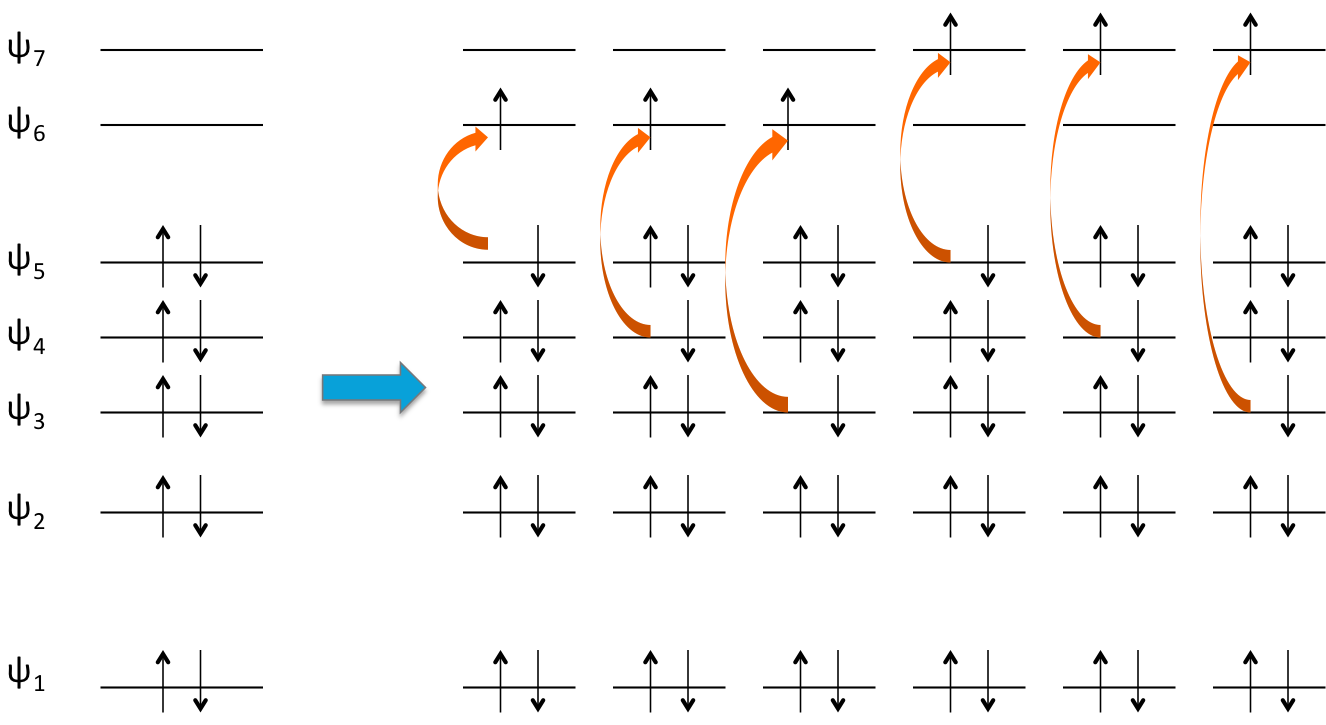
\includegraphics[height=2.0in]{figures/cis.png}
\end{center}
\visible<2->{
\small{
\begin{eqnarray*}
\textcolor{blue}{\Psi_{\textrm{CIS}}^{\textrm{\textcolor{red}{singlet}}} = \sum_{ai} X_{ai} \left[  \frac{1}{\sqrt{2}} \left(\Phi_i^a \textcolor{red}{+}  \Phi_{\bar{i}}^{\bar{a}}  \right) \right]   }   &
\textcolor{blue}{\Psi_{\textrm{CIS}}^{\textrm{\textcolor{red}{triplet}}} = \sum_{ai} X_{ai} \left[  \frac{1}{\sqrt{2}} \left(\Phi_i^a \textcolor{red}{-}  \Phi_{\bar{i}}^{\bar{a}}  \right) \right]   }
\end{eqnarray*}
}
}
\end{frame}


\begin{frame}
\begin{itemize}
\item The CIS wavefunction 
\begin{equation*}
\Psi_{\textrm{CIS}} = \sum_{ai} X_{ai} \Phi_i^a 
\end{equation*}
are obtained by diagonalizing the Hamiltonian in the subspace spanned by all singly-excited configurations. 
\begin{center}
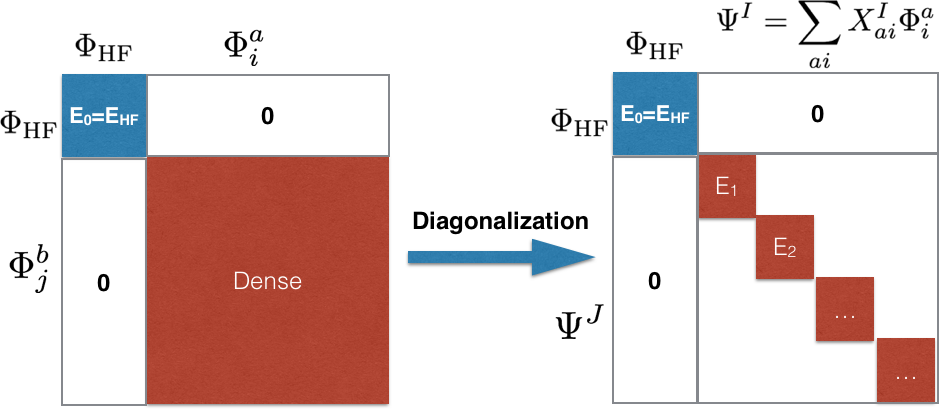
\includegraphics[height=1.5in]{figures/cis-2.png}
\end{center}
\end{itemize}
\end{frame}

\begin{frame}
\begin{itemize}
\item \small{Given the Hamiltonian,}
\begin{eqnarray*}
\hat{H} & = &  \sum_i \left(- \frac{1}{2} \bigtriangledown_i^2  - \sum_A \frac{Z_A}{\left| \vec{r}_i - \vec{R}_A \right| } \right) +  \sum_{i < j} \frac{1}{\left| \vec{r}_{i} - \vec{r}_j \right| }  
\end{eqnarray*}

\item The Hamiltonian matrix elements
\begin{eqnarray*}
\left< \Phi_i^a \middle| \hat{H}  \middle| \Phi_j^b \right>  = E_0 + \left( \varepsilon_a - \varepsilon_i \right) \delta_{ij} \delta_{ab}  + ( a i | b j) - ( a b | i j) 
\end{eqnarray*}
\visible<2->{
\item For singlet configurations
\begin{eqnarray*}
\left< \frac{ \Phi_i^a \textcolor{red}{+} \Phi_{\bar{i}}^{\bar{a}}  } { \sqrt{2}}  \middle| \hat{H}  \middle| \frac{ \Phi_j^b \textcolor{red}{+} \Phi_{\bar{j}}^{\bar{b}}  } { \sqrt{2}}    \right>  
= E_0 + \left( \varepsilon_a - \varepsilon_i \right) \delta_{ij} \delta_{ab} + 2 ( a i | b j) - ( a b | i j)  
\end{eqnarray*} 
}

\visible<3->{
\item For triplet configurations
\begin{eqnarray*}
\left< \frac{ \Phi_i^a \textcolor{red}{-} \Phi_{\bar{i}}^{\bar{a}}  } { \sqrt{2}}  \middle| \hat{H}  \middle| \frac{ \Phi_j^b \textcolor{red}{-} \Phi_{\bar{j}}^{\bar{b}}  } { \sqrt{2}}    \right>  
= E_0 + \left( \varepsilon_a - \varepsilon_i \right) \delta_{ij} \delta_{ab}  - ( a b | i j)  
\end{eqnarray*} 
}

\end{itemize}
\end{frame}

\begin{frame}
\frametitle{Case Study: Water Molecule}
\begin{itemize}
\item \small{Use IQmol to build water molecule (O-H: 0.95 \AA; H-O-H: 105$^\circ$). }
\item Perform CIS calcn's to find two lowest singlet and triplet excited states.  
\end{itemize} 
\begin{center}
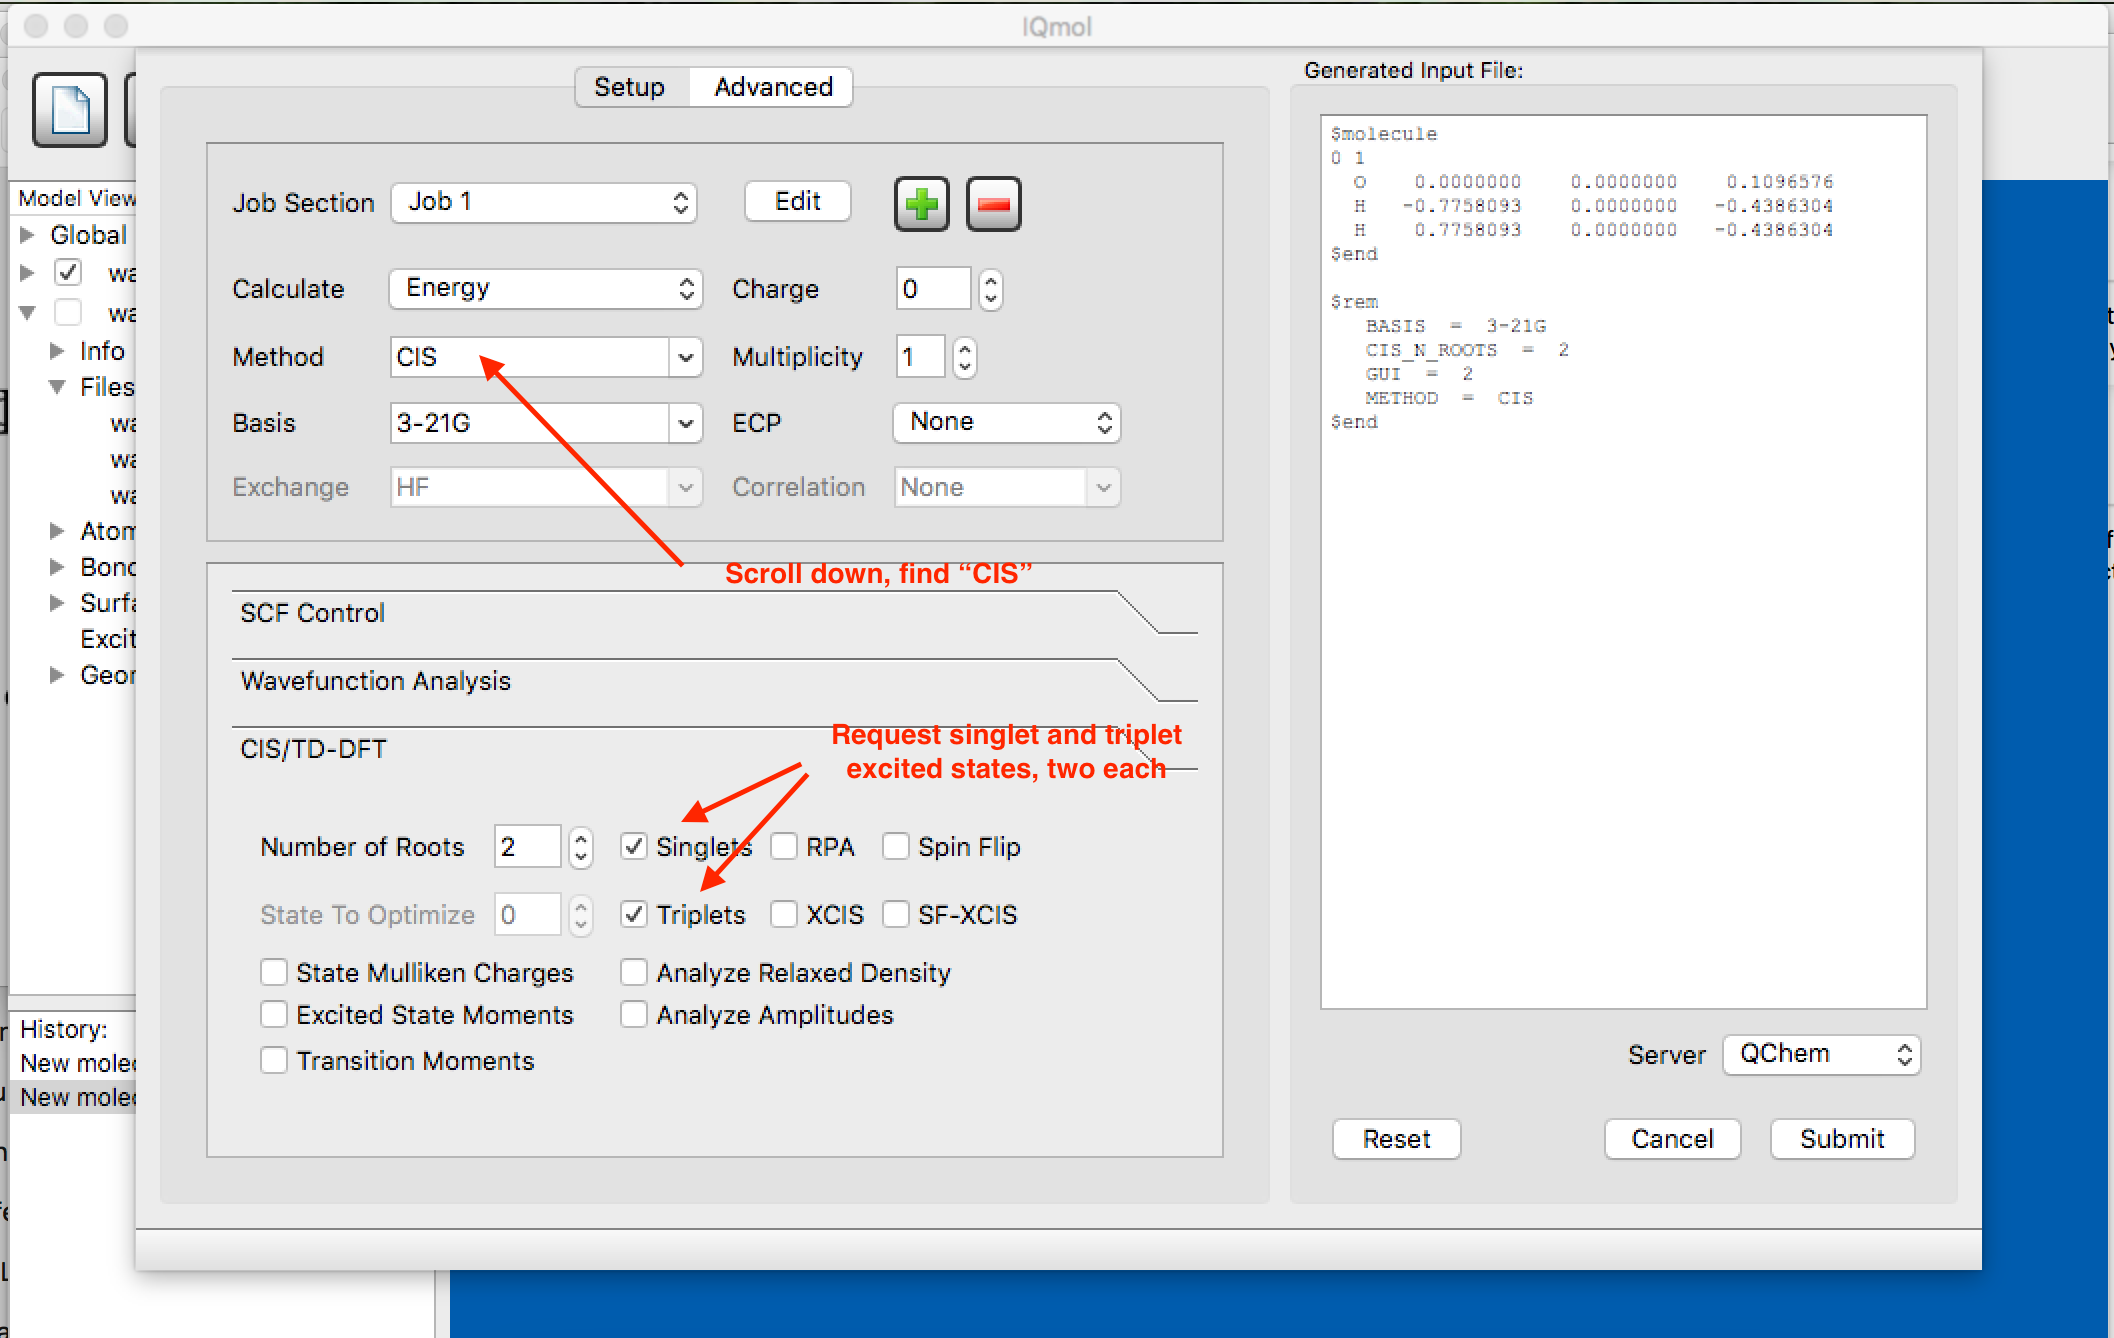
\includegraphics[height=2.0in]{figures/cis-input.png}
\end{center}
\end{frame}

\begin{frame}
\frametitle{Q-Chem Output File} 
\begin{center}
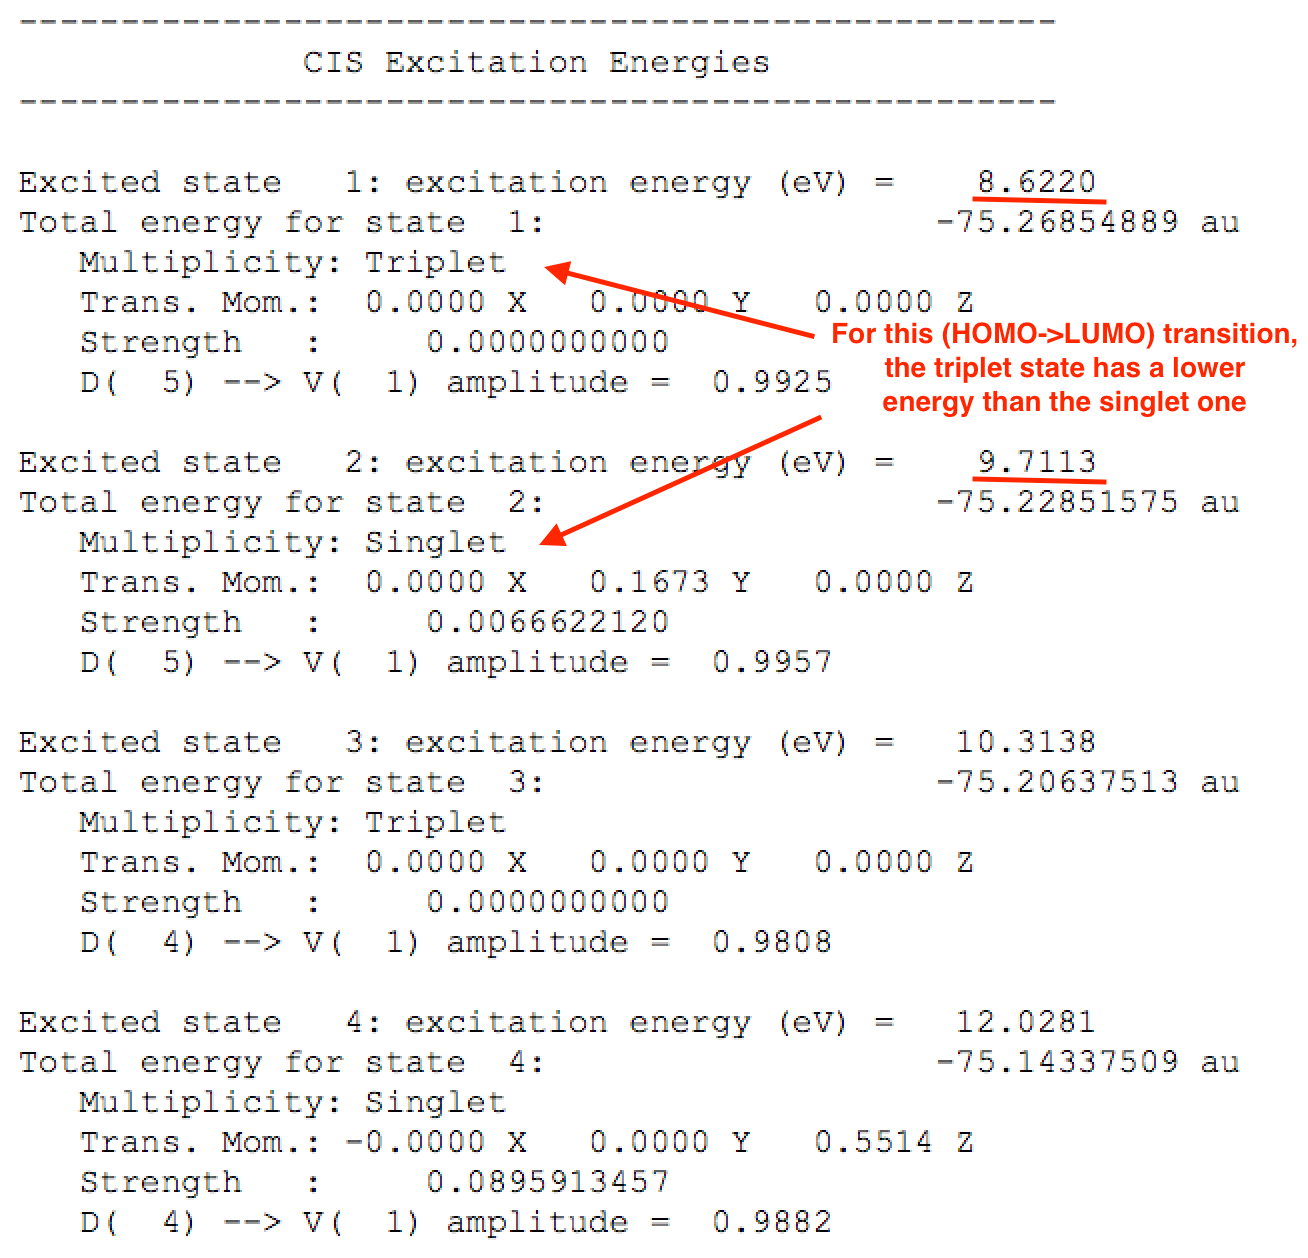
\includegraphics[height=2.8in]{figures/cis-output.png}
\end{center}
\end{frame}

\begin{frame}
\frametitle{Singlet and Triplet Excitation Energies}
\begin{itemize}
\item \small{Copy over}
\begin{itemize}
\item /home/yihan/qm\_tutorial/qchem\_files/FCIDump
\item /home/yihan/qm\_tutorial/python\_files/read\_fcidump.py
\end{itemize}
\item Follow the Hartree-Fock energy code, compute
\begin{itemize} 
\item \footnotesize{singlet/triplet excitation energies for the HOMO $\rightarrow$ LUMO transition}
\item singlet/triplet excitation energies for the HOMO-1 $\rightarrow$ LUMO transition 
\end{itemize}
\end{itemize}
\begin{center}
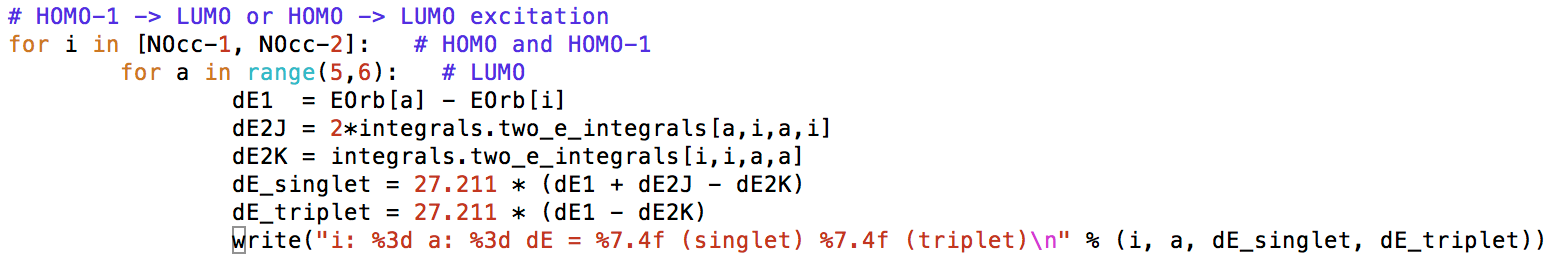
\includegraphics[height=1.2in]{figures/cis-code-1.png}
\end{center}
\end{frame}

\begin{frame}
\begin{itemize}
\item Redo the calculation using actual amplitudes, after copying over
\begin{itemize}
\item /home/yihan/qm\_tutorial/water.cis.amplitudes
\item  /home/yihan/qm\_tutorial/python\_files/matrix\_print.py
\item  /home/yihan/qm\_tutorial/python\_files/read\_amplitudes.py
\end{itemize}
\end{itemize}
\begin{center}
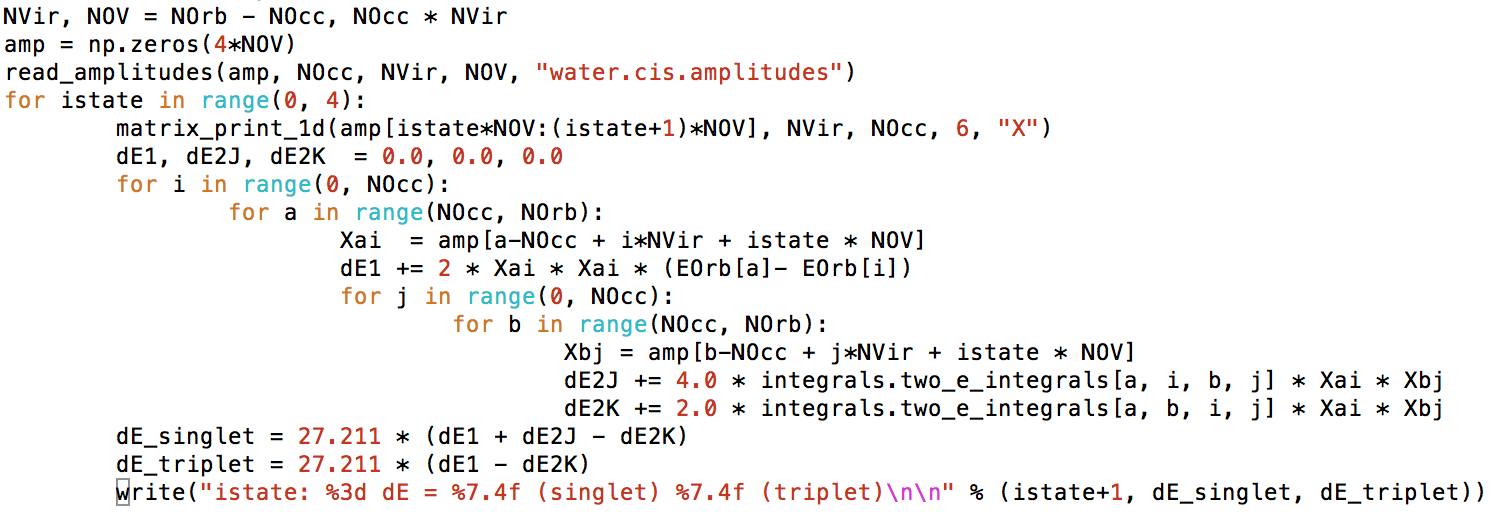
\includegraphics[height=1.6in]{figures/cis-code-2.png}
\end{center}
\end{frame}

\begin{frame}
\begin{itemize}
\item \footnotesize{For a triplet state involving HOMO and LUMO, there are three components:}
\begin{itemize}
\item \footnotesize{S$_z$=0, slide 8} 
\item \footnotesize{S$_z$ =1, -1.   Now let us compute the energy of the S$_z$=1 component.  }
\end{itemize}
\end{itemize}
\begin{center}
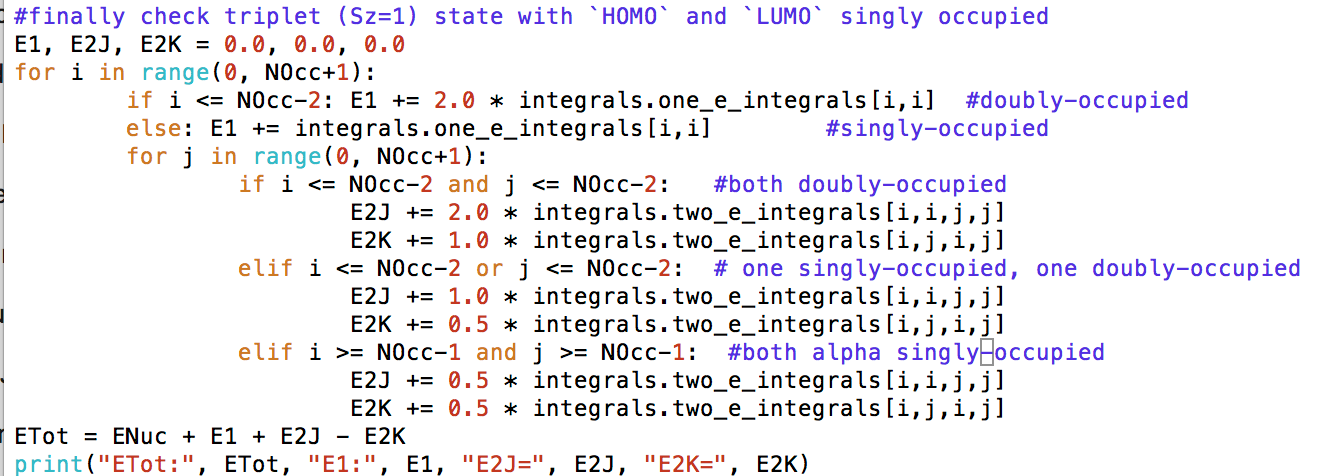
\includegraphics[height=1.6in]{figures/rohf-code.png}
\end{center}
\end{frame}


\end{document}

\begin{frame}
\frametitle{Blank Page}
\begin{columns}
\begin{column}{0.4\textwidth}
\begin{center}
\end{center}
\end{column}
\begin{column}{0.6\textwidth}
\begin{center}
\end{center}
\end{column}
\end{columns}
\end{frame}

